\part{Visualizations}

% ------------------------------------------------------------
% ------------------------------------------------------------
\section{Data Set}
\begin{frame}[allowframebreaks, fragile]
\frametitle{Data Set for Tutorial}
	Data set for this tutorial comes from State of California.  Please download it from \\
	\vspace{5pt}

	\noindent \url{https://chhs.data.ca.gov/Healthcare/Number-of-Selected-Inpatient-Medical-Procedures-Ca/mdt8-gwyw}  \\

	\vspace{5pt}
	\noindent To read it into R, type:
  		\begin{lstlisting}[ basicstyle=\footnotesize ]
data <- read.csv(
  file = "Number_of_Selected_Inpatient_Medical_Procedures__California_Hospitals__2005-2014.csv",
  stringsAsFactors = FALSE
  )
		\end{lstlisting}
\newpage
    \begin{center}
     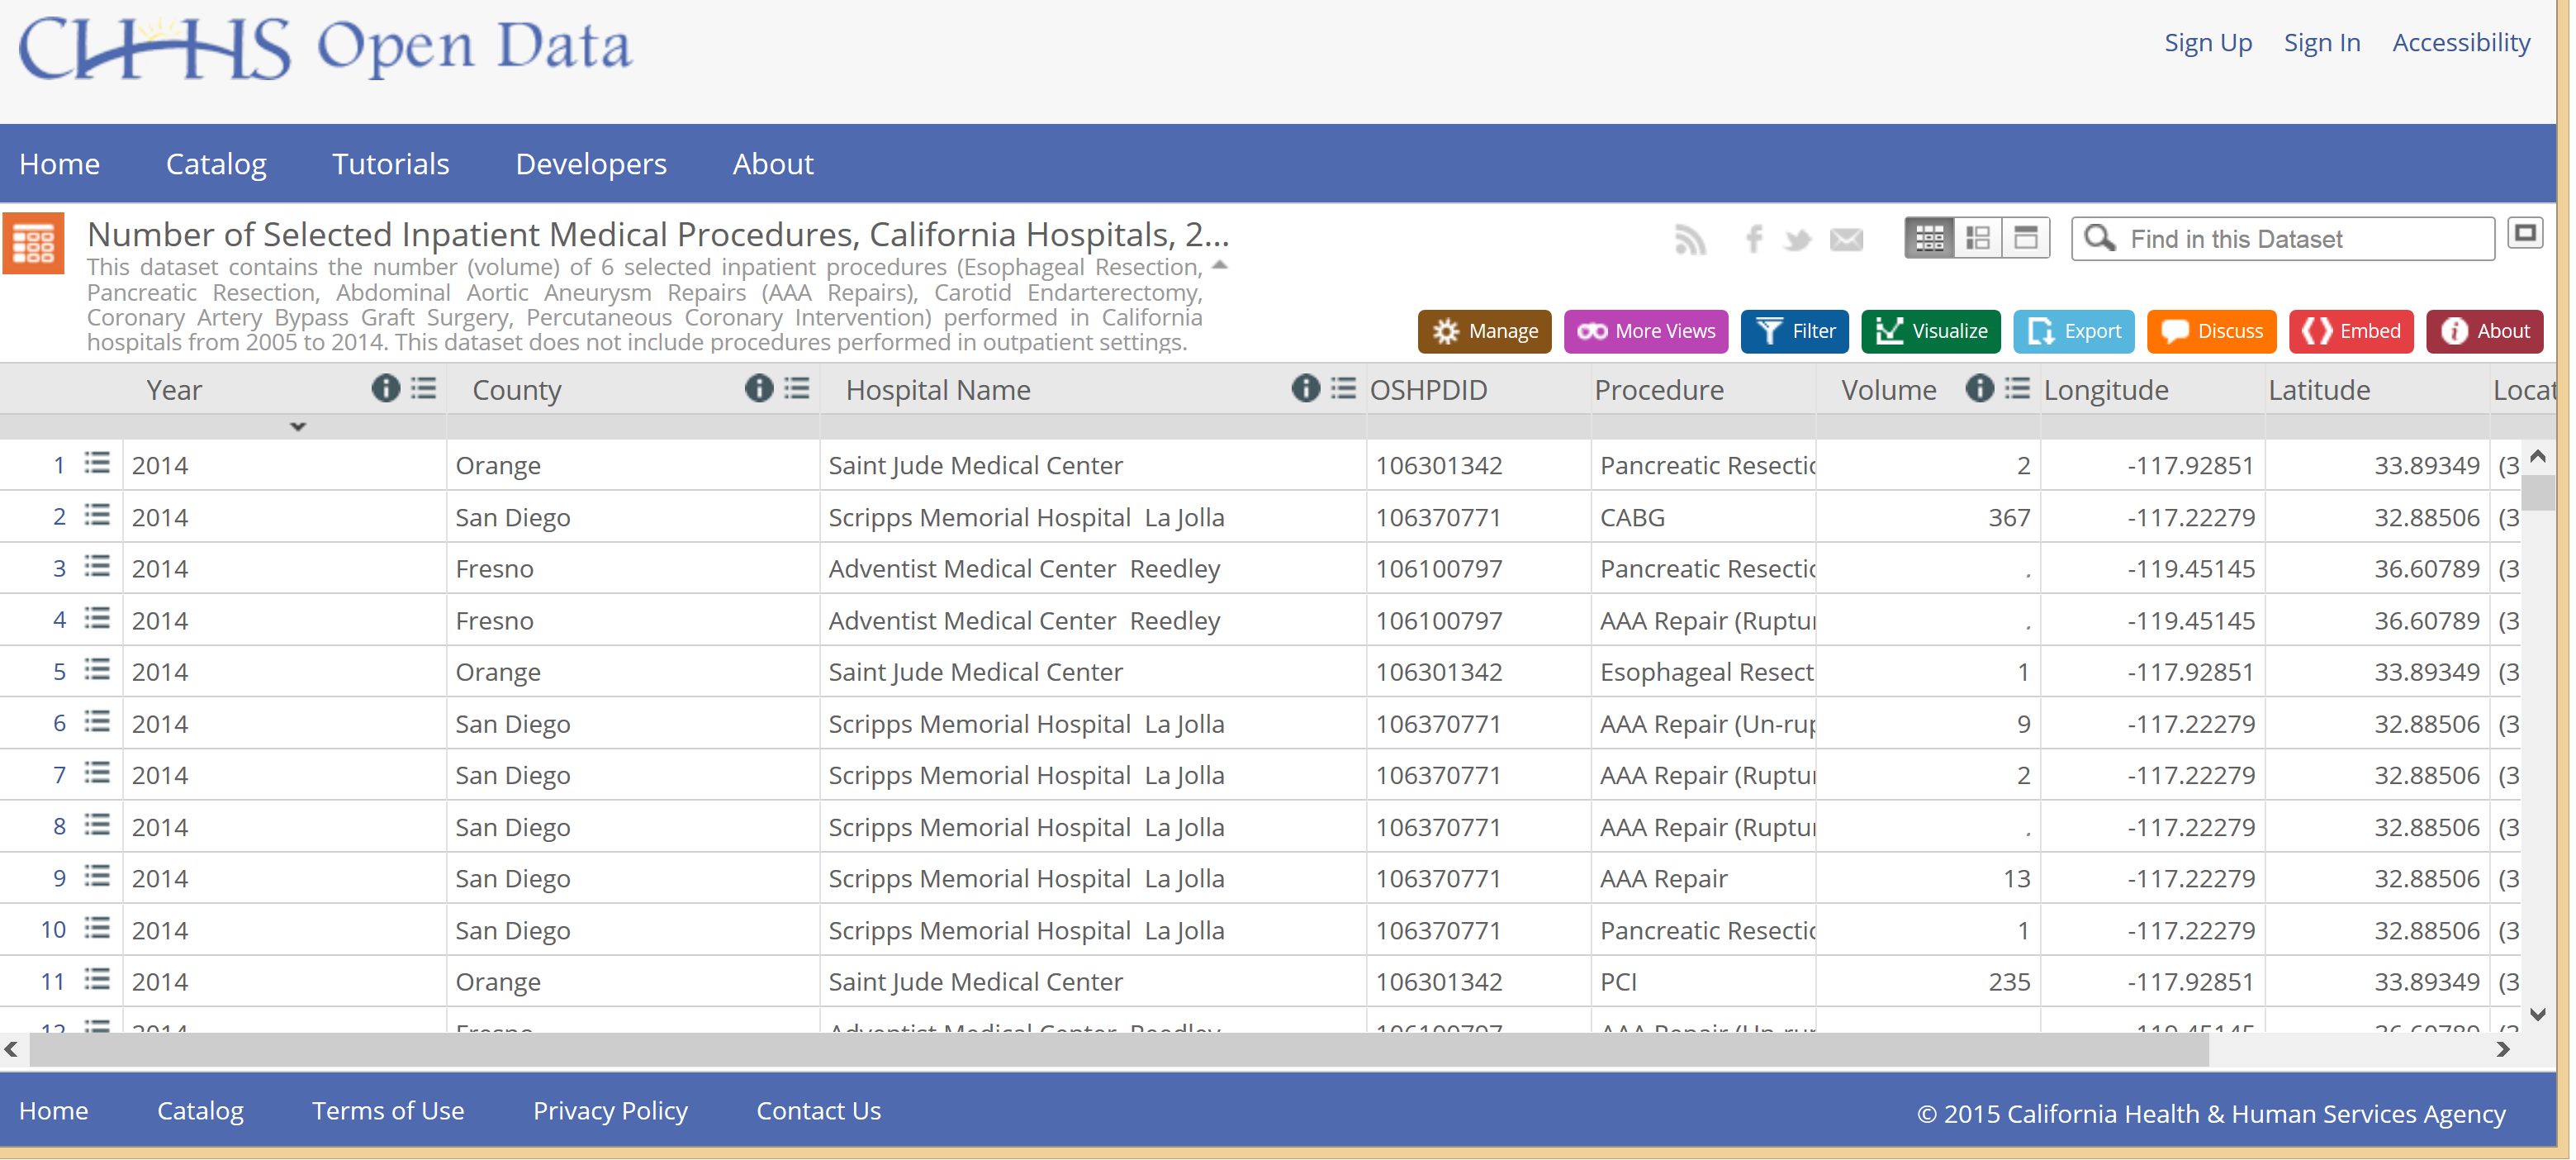
\includegraphics[width=1\textwidth]{images/data.png}
    \end{center}	
\end{frame}


% ------------------------------------------------------------
% ------------------------------------------------------------
\section[Summary Plots]{Summary Plots}

\subsection{Scatterplot}
%%%%% New frame
\begin{frame}[allowframebreaks, fragile]
\frametitle{Scatterplot (v0.1)}

To get a quick peak into the numerical variables in the data \ttfamily scatterplotMatrix(): \normalfont
  		\begin{lstlisting}[ basicstyle=\footnotesize ]
# Load package `car' to use scatterplotMatrix():	
library(car)	
scatterplotMatrix(
  x = data[, c("Latitude", "Longitude", "Volume")], 
  smoother = FALSE, 
  reg.line = FALSE
  )
		\end{lstlisting}
% col=rgb(0.4, 0.2, 0.2, alpha=0.5)

        \begin{center}
         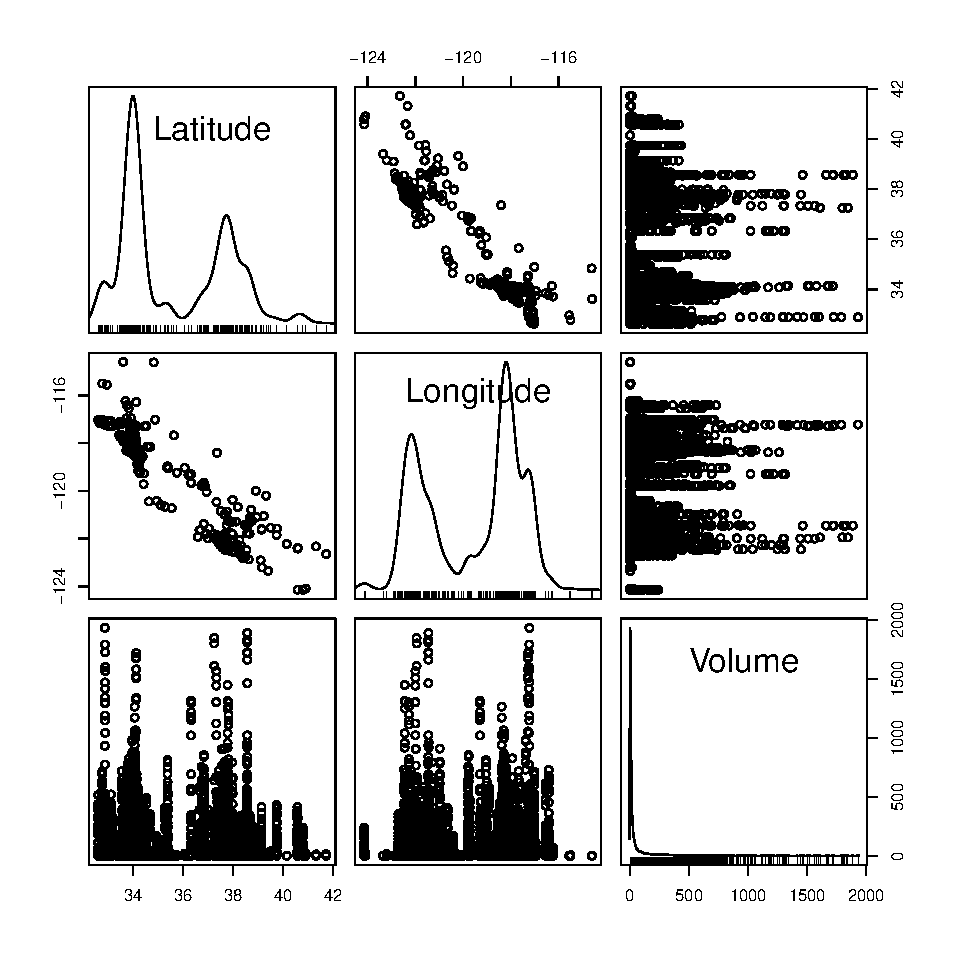
\includegraphics[width=0.63\textwidth]{images/scatterPlot_v0.pdf}
        \end{center}
\end{frame}

\begin{frame}[allowframebreaks, fragile]
\frametitle{Scatterplot (v0.2)}

To get a quick peak into the numerical variables and the trends in the data, modify arguments of \ttfamily scatterplotMatrix(): \normalfont
  		\begin{lstlisting}[ basicstyle=\footnotesize ]
?scatterplotMatrix # for documentation
library(car)		
scatterplotMatrix(
  x = data[, c("Latitude", "Longitude", "Volume")], 
  reg.line = FALSE
  )
		\end{lstlisting}

        \begin{center}
         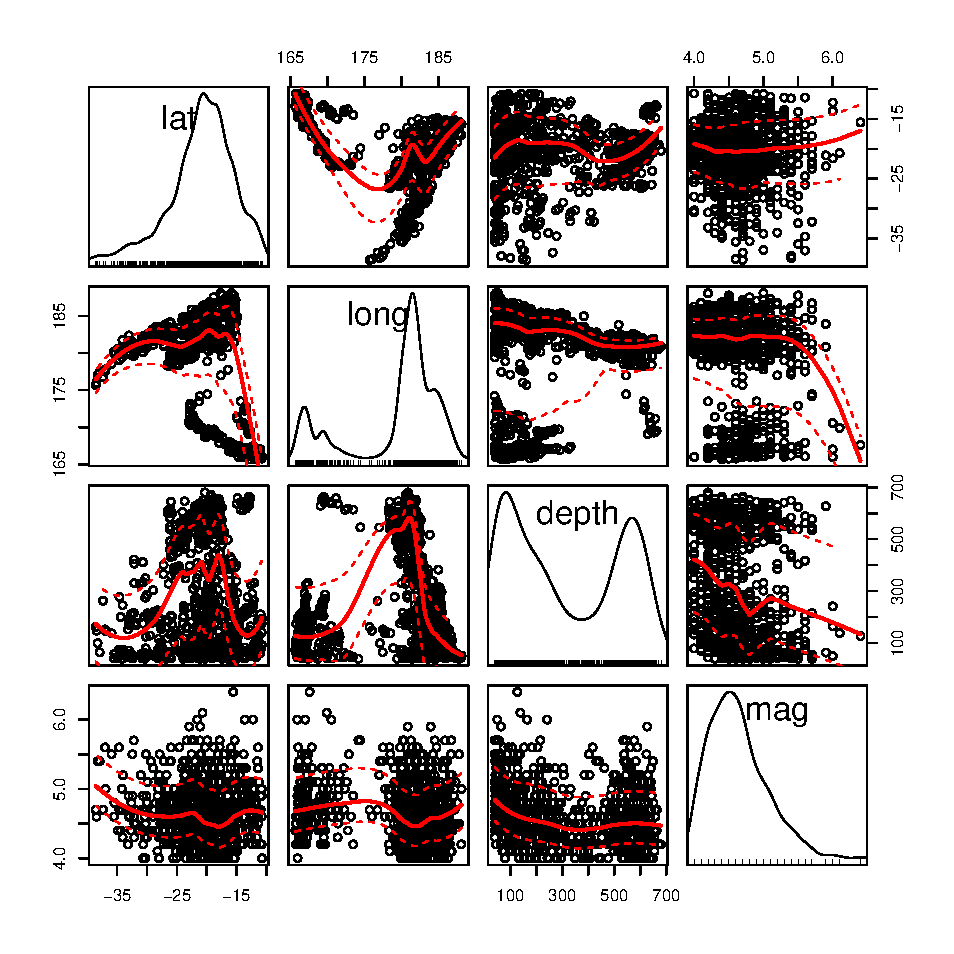
\includegraphics[width=0.63\textwidth]{images/scatterPlot_v1.pdf}
        \end{center}
\end{frame}

\begin{frame}[allowframebreaks, fragile]
\frametitle{Scatterplot (v0.3)}

To improve the color scheme, modify arguments of \ttfamily scatterplotMatrix().  
  		\begin{lstlisting}[ basicstyle=\footnotesize]
library(car)		
scatterplotMatrix(
  x = data[, c("Latitude", "Longitude", "Volume")], 
  reg.line = FALSE,
  col=c(3,
    "orangered",
    rgb(176/256, 196/256, 222/256, alpha=0.5)
    ), 
  pch=19,
  lwd=3
  )
		\end{lstlisting}
\normalfont
\framebreak
You can specify a color in R via: 
\begin{itemize}
	\item Number (e.g. 1 = black, 2 = red, etc.)
	\item Name (e.g. "black", "red", "dodgerblue")
	\item RGB (e.g. c(0,0,0) = black, c(1,0,0) = red, etc.)
	\item Please see \url{http://research.stowers-institute.org/efg/R/Color/Chart/} for color references. 
\end{itemize}

\noindent Note the order of color arguments. \normalfont
        \begin{center}
         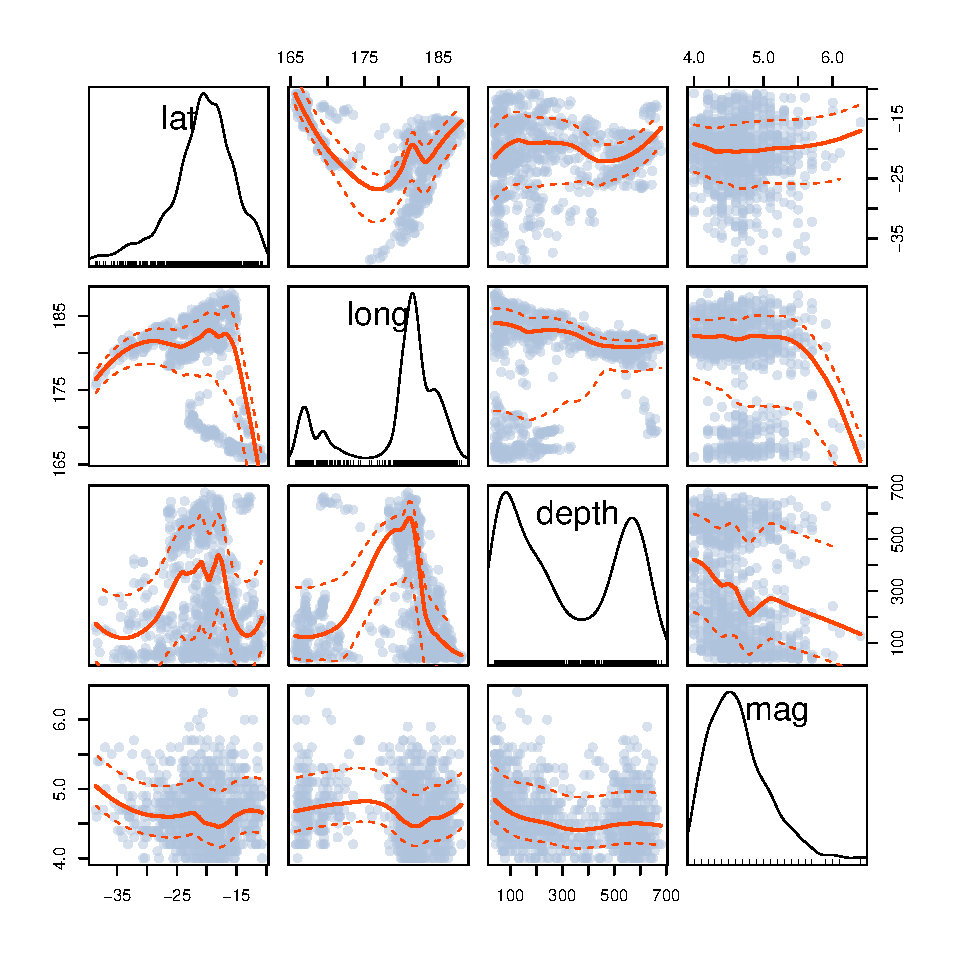
\includegraphics[width=0.63\textwidth]{images/scatterPlot_v3.pdf}
        \end{center}
\end{frame}

% %---
% \begin{frame}[allowframebreaks, fragile]
% \frametitle{Scatterplot (v0.4)}
%   \framesubtitle{Data = Fiji Earthquakes Since 1964}

% Another way to get a quick peak into the numerical variables in the data is via \ttfamily ggpairs(): \normalfont
%   		\begin{lstlisting}[ basicstyle=\small ]
% library(ggplot2)
% library(GGally)
% ggpairs(
% 	data[, c("Latitude", "Longitude", "Volume")]
% 	)
% 		\end{lstlisting}
% % col=rgb(0.4, 0.2, 0.2, alpha=0.5)

%         \begin{center}
%          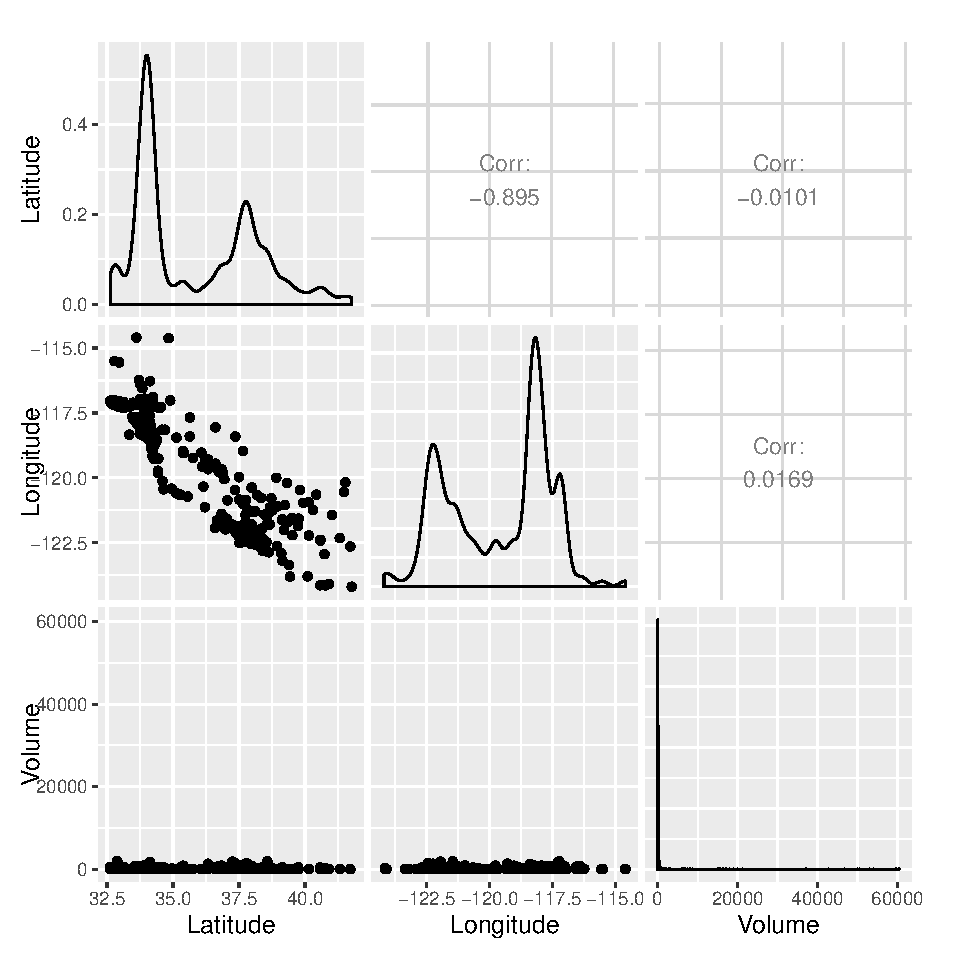
\includegraphics[width=0.6\textwidth]{images/scatterPlot_v4.pdf}
%         \end{center}
% \end{frame}

%%%%% New frame
\subsection{Histogram}

\begin{frame}[fragile, allowframebreaks]
	\frametitle{Histogram}
To compare the distribution of one variable, use use \ttfamily histogram(): \normalfont

\end{frame}

%----
\begin{frame}[fragile, allowframebreaks]
	\frametitle{'Nicer' Histogram}

To compare the frequencies of two variables side-by-side, use \ttfamily beanplot(): \normalfont

	\begin{lstlisting}[ basicstyle=\tiny ]
library(beanplot)
op <- par(las=2)
beanplot(
  Volume ~ as.factor(County), 
  data = data_LA_SF, 
  xlab = "",
  log = "y",
  side = "both", 
  col = list( c( grey(0.5), "white"), grey(0.8) ), 
  border = NA, 
  overallline = "median", 
  ll = 0.005
  )
legend(
  x = "bottomleft",
  fill=c( grey(0.5), grey(0.8) ), 
  legend=c( "LA", "SF" )
  )
par(op)
	\end{lstlisting}

        \begin{center}
	         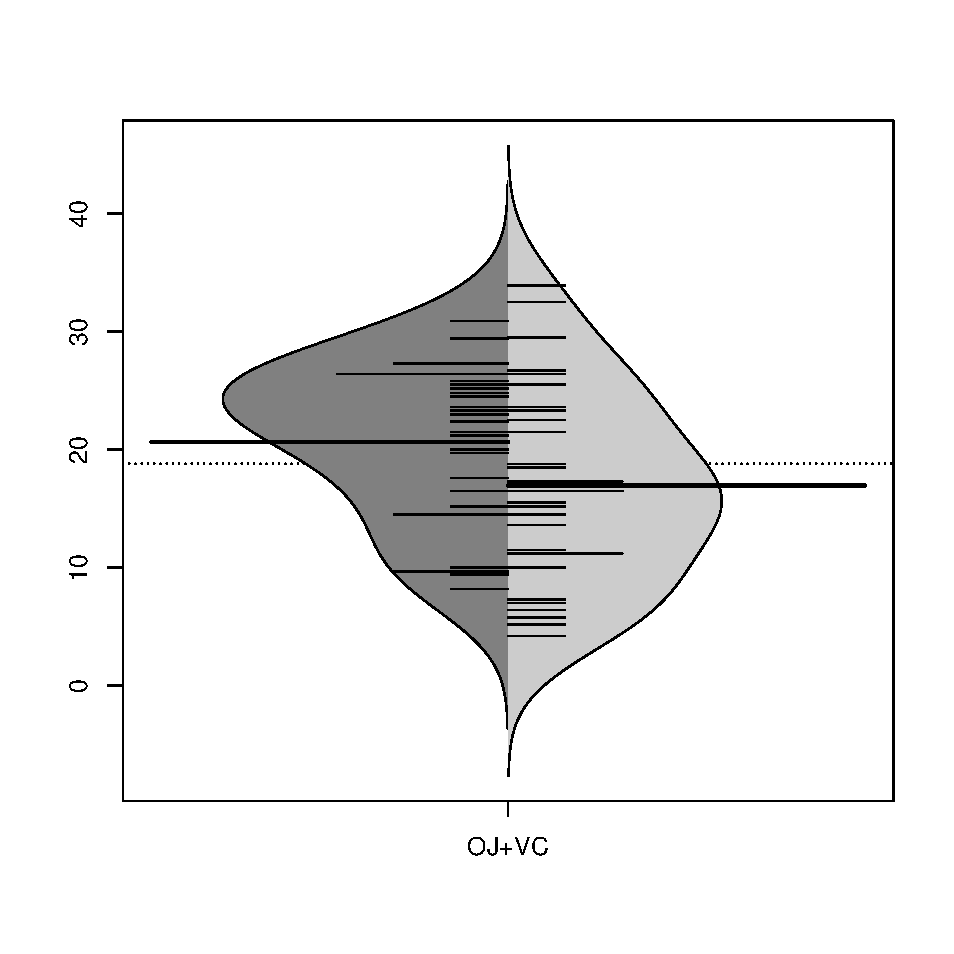
\includegraphics[width=0.65\textwidth]{images/beanplot_v0.pdf}
        \end{center}

\end{frame}


%%% NOT WORK...
%
%library(lattice)
%split.screen(c(1,2))        # split display into two screens
%split.screen(c(2,1),2)      # split bottom half in two
%screen(1)                   # prepare screen 1 for output
%qqplot(ToothGrowth$len~ToothGrowth$supp)
%screen(4)                   # prepare screen 4 for output
% # boxplot(ToothGrowth$len~ToothGrowth$supp)
% beanplot(ToothGrowth$len~ToothGrowth$supp, col=list(grey(0.5),c(grey(0.8),"white")), border = NA, overallline = "median", ll=0.01, side="both")
%screen(1, FALSE)            # return to screen 1, but do not clear
%close.screen(all = TRUE)    # exit split-screen mode


%%%%%%%%%%%%%%%%%%%%%%%%%%%%%%%%%%%%%

% ------------------------------------------------------------
% ------------------------------------------------------------

% Exercise: compare distributions of Iris data
% ID outlier in dataset

\subsection{Exercise I}
\begin{frame}
	\frametitle{Exercise I}
	Compare the distributions of the sepal widths for the three species of irises (using the \ttfamily iris \normalfont data set).
\end{frame}